\documentclass[]{article}
\usepackage[english]{babel}
\usepackage{amsmath}
\usepackage{graphicx}
\usepackage[hypcap=false]{caption}
\usepackage{subcaption}
\graphicspath{ {./images/} }
\usepackage{hyperref}
\hypersetup{
	hidelinks
	}

\title{Artificial Intelligence in Cybersecurity: Assignment 5}
\author{Brandon Hosley}
\date{\today}

\begin{document}
	\maketitle
	
\section{Introduction}

In this article \cite{Vien2021} outlines a proposal to use machine learning to improve and secure the transmission of images over a public space.
The team utilizes machine learning in the form of Convolutional Neural Networks (CNNs) for both the down-sampling of high-resolution images and up-sampling low-resolution images.
For the transmission portion the team use a steganographic method that they erroneously refer to as stenography for the majority of the paper, except when the authors refer to the carrier images loaded with the data to be secured as 'stegos'.

\section{Data Sources}

% Describe the data used in this paper including source, sample, attribute, etc. (10 points)
The data utilized for this paper was sourced from \cite{Grubinger2006}.
This dataset consists of a large number of photos collected for the 
CLEF cross-language image retrieval track (ImageCLEF).
The dataset is assembled from 20,000 images from a private collection.
It was originally used for pattern recognition, but for this paper the images are utilized as both samples for the carried data and as the data carrier.

\section{Algorithm}

% Explain the algorithm/method for visualization in detail from your understanding (20 points)


% Draw a flowchart of the algorithm for visualization (10 points)
\begin{figure}[h]
	\centering
	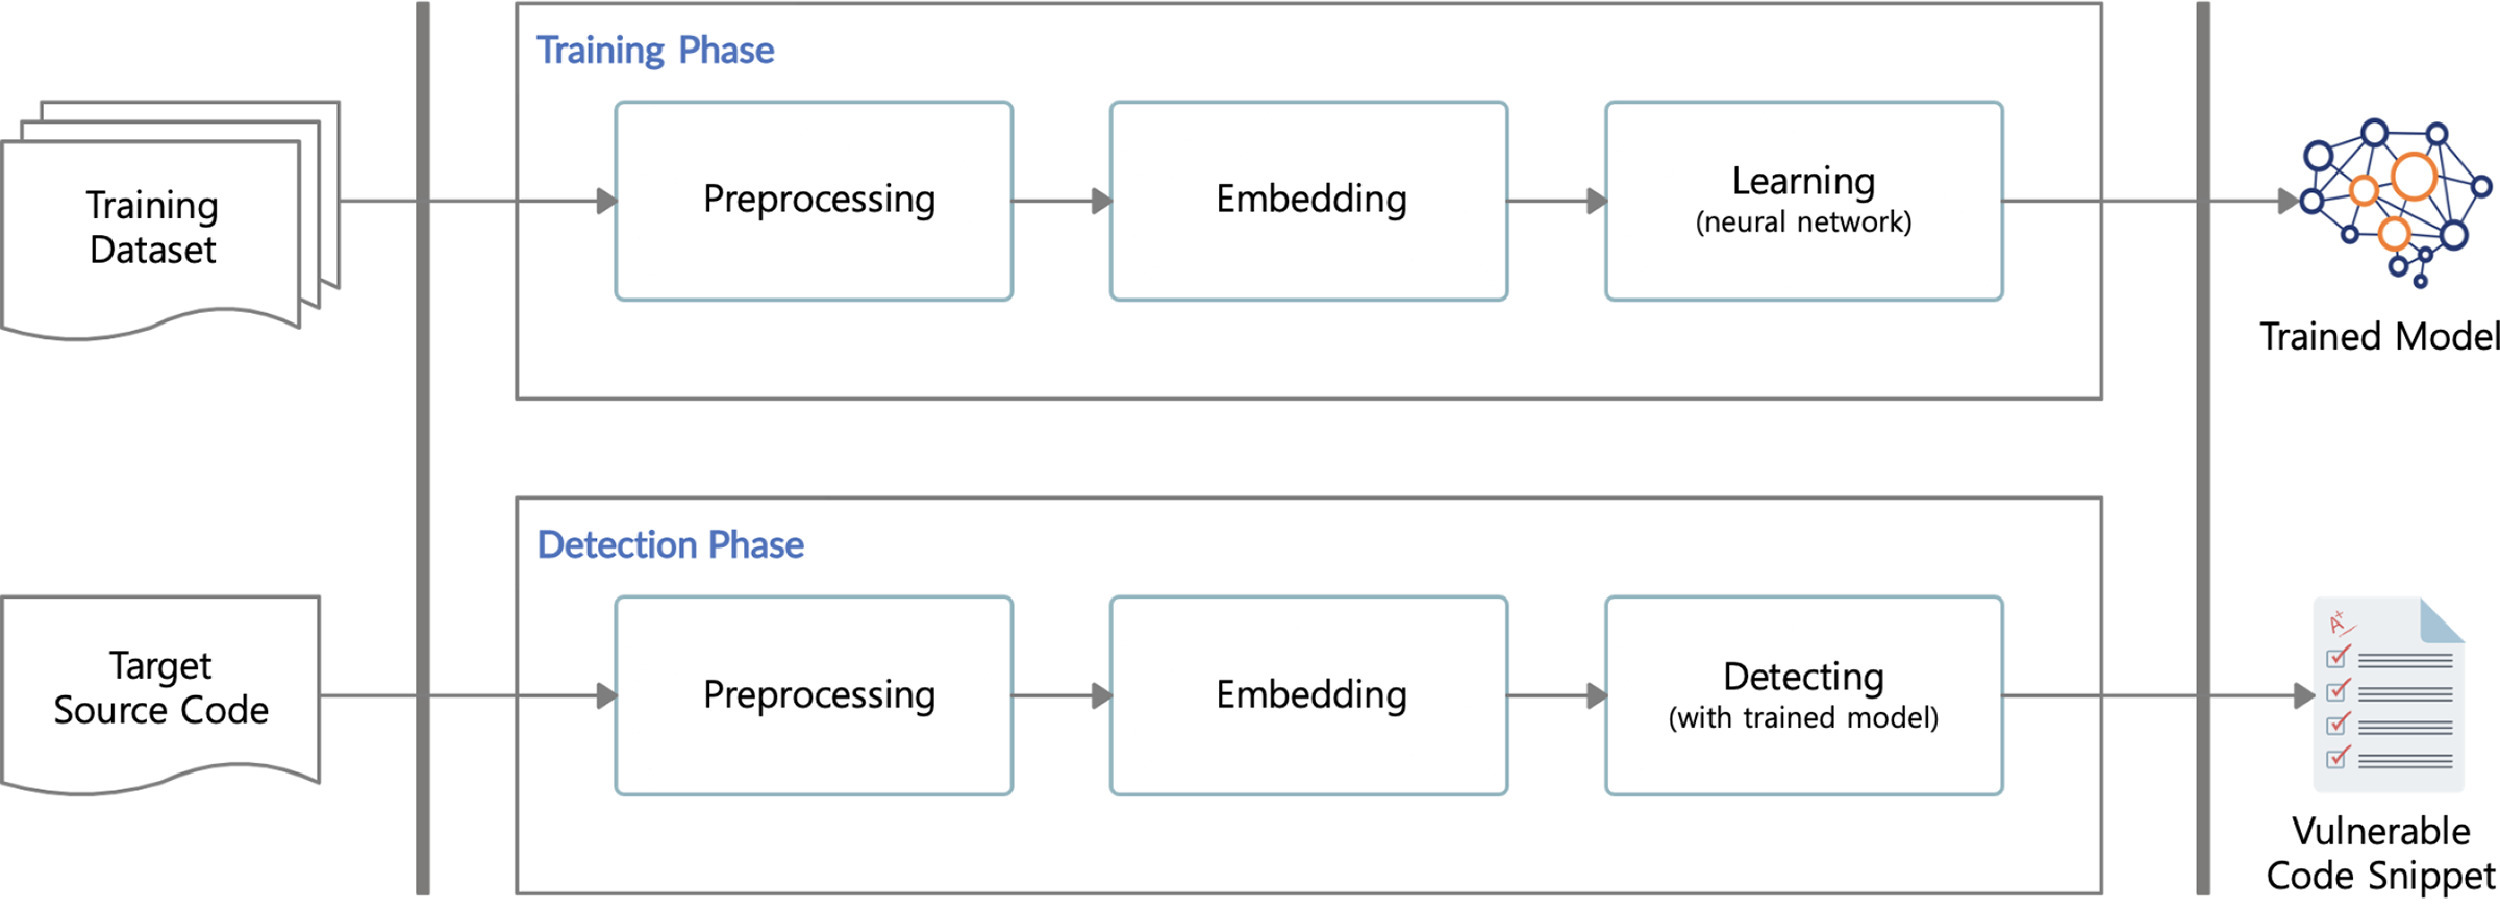
\includegraphics[width=0.8\textwidth]{Algorithm}
	\caption{Deep-NC \cite{Vien2021}}
\end{figure}


\section{Results}

% Explain the experimental results in detail from your understanding (10 points)
The research team successfully demonstrated the capability of their framework to accomplish what they had intended for it to accomplish. Their steganographic method with CNN enabled upsampling was able to achieve a 32 db PSTN (Peak Signal To Noise) ratio when compared to an eavesdropper.

\section{Advantages and Disadvantages}

% Discuss the advantages from your understanding (10 points)


% Discuss the disadvantages from your understanding (15 points)


\section{Improvements}

% Provide the specific ideas to improve the algorithm. General ideas are not allowed. (15 points)



\clearpage
\bibliographystyle{acm}
\bibliography{\jobname}
\end{document}